\chapter{Le premier principe de la thermodynamique} 
Également connu sous le doux nom de \textit{principe de 
conservation de l'énergie}, il s'agit d'un postulat fondamental
qui ne se démontre pas.

\section{Transformations fermées (cycles) d'un système fermé}
Soit le système fermé ci-dessous :
\begin{center}
	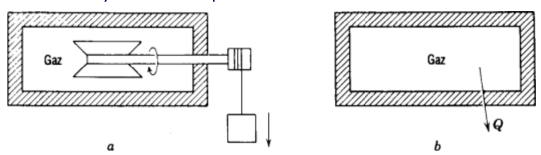
\includegraphics[scale=0.5]{ch5/image1}
	\captionof{figure}{ }
\end{center}
On travaille en deux temps :
\begin{enumerate}
	\item On fournit un travail $W$ au système.
	\item On le laisse revenir à son état initial par échange de $Q$.
\end{enumerate}
Ces deux transformations constituent un cycle. Le premier principe 
postule que\\

\retenir{Le travail $W$ et la chaleur $Q$ échangés au cours d'un 
	tel cycle sont proportionnels, la constante de proportionnalité 
	étant toujours la même.
	\begin{equation}
		JQ = W \qquad \Leftrightarrow \qquad J\oint \delta Q = \oint \delta 
		W
	\end{equation}
	où $J$, la constante de $\propto$ dépend des unités utilisées.}\ \\

Si $Q$ et $W$ sont dans la même unité, cette constante vaut -1 et 
l'expression du premier principe devient
\begin{equation}
	\oint (\delta Q + \delta W) = 0
\end{equation}

\section{Transformation ouvertes d'un système fermé}
Soit un système fermé subissant un cycles formé de deux transformations 
successives $A$ et $B$. En vertu du premier principe :\\
\begin{wrapfigure}[9]{l}{6cm}
	\vspace{-7mm}
	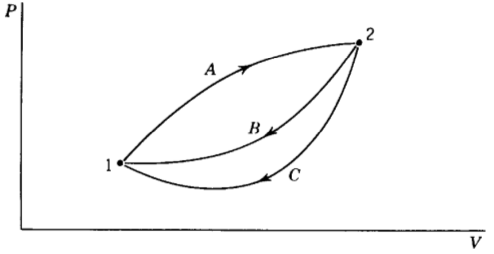
\includegraphics[scale=0.34]{ch5/image2.png}
	\captionof{figure}{ }
\end{wrapfigure}
\vspace{-1cm}
\begin{equation}
	\oint (\delta Q + \delta W) = \int_1^2 (\delta Q + \delta W)_A + \int_2^1 
	(\delta Q + \delta W)_B = 0
\end{equation}
De même, pour le cycle formé par $A$ et $C$ :
\begin{equation}
	\int_1^2 (\delta Q + \delta W)_A + \int_2^1 (\delta Q + \delta W)_C = 0
\end{equation}
Par soustraction, en en déduit que
\begin{equation}
	\int_1^2 (\delta Q + \delta W)_B = \int_1^2 (\delta Q + \delta W)_C
\end{equation}
Les chemins $B$ et $C$ sont arbitraires, l'intégrale est indépendante 
du chemin parcouru : $(\delta Q + \delta W)$ est une différentielle 
exacte que l'on désigne :
\begin{equation}
	dE = \delta Q + \delta W
\end{equation}
où $dE$ est l'\textbf{énergie du système}. En intégrant de l'état 1 à 
l'état 2, on obtient
\begin{equation}
	\ _1Q_2 + \ _1W_2 = E_2-E_1
\end{equation}
Cette énergie peut être cinétique, potentielle, chimique, \dots En 
thermodynamique, on sépare les énergies cinétiques et potentielles 
des autres\footnote{Car elles dépendent du référentiel et s'expriment 
	en fonction de la masse, de la vitesse et des coordonnées dans ce 
	référentiel.} qui sont regroupées dans une variable $U$, l'\textbf{
énergie interne}.
\begin{equation}
	dE = dU + dE_{cin.} + dE_{pot.}
\end{equation}
La forme différentielle du premier principe s'exprime :
\begin{equation}
	\delta Q + \delta W = dU + dE_{cin.} + dE_{pot.}
\end{equation}
Après substitution des expression bien connue grâce aux cours de \textit{
Mécanique rationnelle I/II} : 
\begin{equation}
	\delta Q + \delta W = d\left(\frac{mc^2}{2}\right) + d(mgz)
\end{equation}
En intégrant entre les états initial et final (si $g$ est constante)
\begin{equation}
	\ _1Q_2 + \ _1W_2 = U_2 - U_1 + m\frac{c_2^2-c_1^2}{2}+mg(z_2-z_1)
\end{equation}
Ces équations n'informent que sur les variations d'énergie qui sont 
donc définie à une constante près.

\section{L'énergie interne}
La variable $U$ est extensive et on peut dès lors lui associer une 
variable extensive, l'énergie interne massique $u$. Comme on peut 
décrire l'état d'une substance pure par deux variables indépendantes, 
l'énerge interne est liée aux auters variables par une relation d'état 
ce pourquoi cette grandeur apparaît à côté d'autres variables dans les 
tables.\\
En zone de saturation, on lie $U$ au titre vapeur et massique :
\begin{equation}
U = U_l+U_g \qquad\rightarrow\qquad mu = m_lu_l + m_gu_g
\end{equation}
En divisant par la masse $m$
\begin{equation}
u = (1-x)u_l + xu_g = u_l + x(u_g-u_l)
\end{equation}

\section{Analyse de problème}
Voici la sainte marche à suivre en TP pour réussir son examen. Il 
faut apporter une réponse à : 
\begin{enumerate}
\item Quel est le système ? Tracer les frontière. Ouvert? Fermé ?
\item État initial ? État final ?
\item Transformations ? Variables constantes ?
\item Utile de représenter la transformation ?
\item Quel modèle décrit cette substance\footnote{Une erreur fréquente 
est d'utiliser un modèle de gaz parfait $U(T)$ pour un changement de 
phase (variation de $U$, mais pas de $T$).}
\item Échangés aux frontières ?
\item Stratégie à adopter ?
\end{enumerate}

\section{L'enthalpie}
\begin{wrapfigure}[9]{l}{4.2cm}
	\vspace{-7mm}
	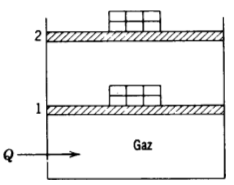
\includegraphics[scale=0.5]{ch5/image3.png}
	\captionof{figure}{ }
\end{wrapfigure}
Soit une transformation quasi-statique isobare d'un système fermé. Par 
le premier principe
\begin{equation}
\ _1Q_2 + \ _1W_2 = U_2-U_1
\end{equation}
Comme c'est une transformation quasi-statique d'un système fermé à 
frontière mobile ($p=cste$) :
\begin{equation}
\ _1W_2 = -\int_1^2 pdV = -p(V_2-V_1)
\end{equation}
Par substitution
\begin{equation}
\ _1Q_2 = U_2-U_1 + p(V_2-V_1) - (U_2+p_2V_2)-(U_1+p_1V_1)
\end{equation}
La chaleur échangée est ici égale à la variation de $U+pV$ qui, comme 
constitué de variables d'état est une variable d'état, l'\textbf{
enthalpie} :
\begin{equation}
H \equiv U + pV,\qquad h = u +pv.
\end{equation}
La quantité de chaleur échangée par une transformation isobare quasi-
statique est égale à la variation d'enthalpie. L'enthalpie n'a de 
sens physique que dans ce cas, mais son expression est toujours 
valable. Dans la zone de saturation, l'enthalpie massique dépend lui 
aussi du titre en vapeur :
\begin{equation}
h = (1-x)h_l + xh_g = h_l+x(h_g-h_l)
\end{equation}

\section{Les chaleurs massiques à volume constant et à pression 
constante}
Les chaleurs massiques sont des \textit{coefficients thermodynamiques} : 
des dérivées partielles de variables primaires par rapport à d'autres. 
Ce sont des variables d'état. \\
La chaleur massique à volume constant vaut
\begin{equation}
c_v = \left(\frac{\partial u}{\partial T}\right)_v = \left(\frac{\delta 
q}{\delta T}\right)_v
\end{equation}
où $v$ signifie à volume massique constant. C'est bien une variable 
indépendante de $T$ : on a deux variables indépendantes, ce qui est 
nécessaire pour décrire une substance pure.\\
Il est possible d’interpréter physiquement cette grandeur (d'où la 
seconde égalité ci-dessus):
\begin{equation}
du = \delta q + \delta w = \delta q - pdv = \delta q
\end{equation}
On peut semblablement définir la chaleur massique à pression constante :
\begin{equation}
c_p = \left(\frac{\delta q}{\delta T}\right)_p = \left(\frac{\delta h}{
\delta T}\right)_p
\end{equation}
Quelques remarques (trois, pour être précis)
\begin{enumerate}
\item Comme ce sont des variables d'état, elles sont indépendantes de 
la transformation (fournir 100J de travail ou chaleur est équivalent)
\item Elles ne concernent que le travail de compression.
\item Pour les solides $pv \rightarrow 0 : c_p\approx c_v$. De plus, 
pour pas mal de transfo. on peut admettre que la chaleur massique est 
constante afin d'avoir
\begin{equation}
h_2-h_1\approx h_2-u_1 = c(T_2-T_1)
\end{equation}
\end{enumerate}


\section{L'énergie interne, l'enthalpie et les chaleurs massiques des 
gaz parfaits}
\begin{wrapfigure}[8]{r}{5.8cm}
	\vspace{-12mm}
	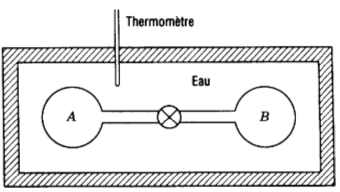
\includegraphics[scale=0.5]{ch5/image4.png}
	\captionof{figure}{ }
\end{wrapfigure}
Joule avec l'\textit{expérience de Joule} (sisi j'te jure) a découvert 
une relation liant $U$ aux autres variables.\\
Considérons deux récipient connectés par une vanne, immergés dans un 
réservoir d'eau isolé. $A$ est rempli d'un gaz à haute pression, $B$ 
est vide et on attend l'équilibre thermique. Une fois que c'est le cas, 
on ouvre la vanne pour avoir égalité des pression :\\
\begin{itemize}
\item[$\bullet$] La transfo du système gaz s'effectue sans échange de 
$W$.
\item[$\bullet$] Durant la transfo. $T_{eau}$ ne varie pas : pas d'
échange de chaleur
\end{itemize}\ 

Du fait que $T_{eau}$ soit inchangée, c'est pareil pour $T_{gaz}$ au 
cours de la transfo $\rightarrow$ pas de chaleur échangée, pas de 
travail échangé ; pas de variation d'énergie interne. $U_{gaz}$ ne 
dépend pas de la pression, mais \textbf{uniquement} de $T$ : $u = f(T)$.

\corollaire{\ 
\begin{itemize}
\item Les chaleurs massiques à volume constant ne sont fonction que de 
$T$.
\item L'enthalpie n'est fonction que de $T$.
\item La chaleur massique à pression constante n'est fonction que de $T$.
\end{itemize}} \ \\

$U$ est soumise à plusieurs contributions dues au mouvement des 
molécules et de leur nuage électronique. On parle ici des degrés de 
\begin{description}
\item[Translation] $e_{tr} = \frac{3}{2}RT$
\item[Rotation] $e_{rot} = RT\left(1-\frac{\theta-R}{\theta_R+3T}\right)
$ où $\theta_R$ est la température de rotation de la molécule.
\item[Vibration] $e_{vib} = R_s\frac{\theta_V}{e^{\frac{\theta_V}{T}-1}}$ 
où $\theta_V$ est la température de vibration de la molécule.
\item[Nuage électronique] Pas d'expression analytique simple : 
expérimental.
\end{description}\ 

\begin{wrapfigure}[12]{l}{7.0cm}
	\vspace{-5mm}
	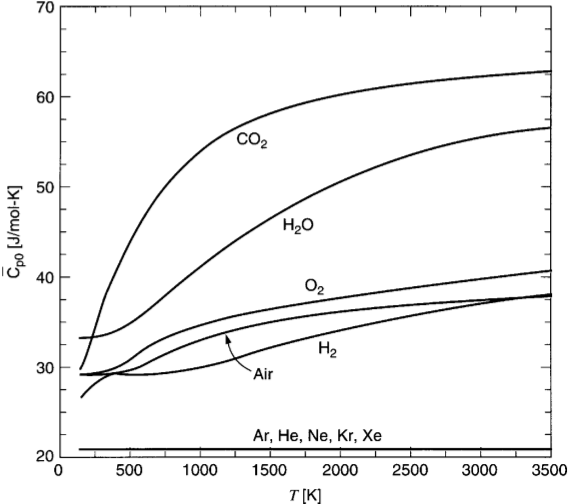
\includegraphics[scale=0.35]{ch5/image5.png}
%	\captionof{figure}{ }
\end{wrapfigure}
Pour la plupart des gaz, $\theta_R$ est très faible : $e_{rot}\approx RT$. 
L'hydrogène est cependant une exception. Les température de vibration 
pour une molécule diatomique est en général bien plus élevé que la 
température ambiante, impliquant une énergie vibrationnelle nulle. 
Toujours à température ambiante, le nuage électronique est dans son 
état fondamental et ne joue pas.
\begin{itemize}
\item Gaz monoatomiques : $\overline{c_p} = \frac{5}{2}\overline{R}$
\item Gaz diatomiques : $\overline{c_p} = \frac{7}{2}\overline{R}$
\item Gaz polyatomiques : $\overline{c_p} > \frac{7}{2}\overline{R}$
\end{itemize}
Rappelons que pour un gaz parfait, $c_p=c_v+R$.\\

Pour les applications, trois choix :
\begin{enumerate}
\item On considère les chaleurs massiques constantes (bien pour les gaz 
monoatomiques).
\item On utilise une relation empirique.
\item On utilise les tables.
\end{enumerate}

\section{Le premier principe sous la forme d'une équation d'évolution 
temporelle}
Divisons la forme différentielle du premier principe $\delta Q + \delta 
W = dU + dE_{cin.} + dE_{pot.}$ par $dt$, le temps infinitésimal entre 
deux états successif :
\begin{equation}
\frac{d}{dt}\left(U + E_{cin.} + E_{pot.}\right) = \frac{\delta Q}{dt} 
+\frac{\delta W}{dt} = \dot{Q}+\dot{W}
\end{equation}
où $\dot{Q}$ et $\dot{W}$ sont les taux de transfert de chaleur et la 
puissance fournie au système.

\section{Conservation de la masse pour les systèmes ouverts}
Aux facteurs relativistes près, la masse est constante. On va en 
déduire les implications sur un système ouvert en général. La frontière 
de celui-ci \textbf{est une surface fermée} dont certaines parties 
peuvent être mobiles et/ou être le siège d'échange de chaleur, travail 
avec le milieu extérieur.\\
\begin{wrapfigure}[13]{l}{6cm}
%	\vspace{-7mm}
	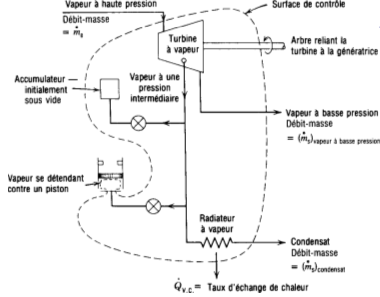
\includegraphics[scale=0.43]{ch5/image6.png}
	\captionof{figure}{ }
\end{wrapfigure}
Soit le système fermé $F$ constitué de la matière dans le système 
ouvert $O$ au moment initial : système fermé $\rightarrow$ masse cste. 
Comme $m_F = \int_{V_F} \rho dV$, on a
\begin{equation}
\frac{dm_F}{dt} = \frac{d}{dt}\int_{V_F} \rho dV = 0
\end{equation}
On peut utiliser les règles dérivatives d'intégrales :
\begin{equation}
\frac{dm_F}{dt}=\frac{d}{dt}\int_{V_F}\rho dV = \int_{V_F}\frac{\partial 
\rho}{\partial t}dV + \oint_{S_F} \rho\vec{b}_F.\vec{n}\ dS = 0
\end{equation}
où $\vec{b}_F$ est le vecteur vitesse de déplacement de la frontière 
du volume $V_F$ : cette vitesse est celle de la matière, $c$, le système 
étant fermé.\\
Similairement, la dérivée par rapport au temps de la masse dans le 
système ouvert $O$ vaut 
\begin{equation}
\frac{dm_O}{dt}=\frac{d}{dt}\int_{V_O}\rho dV = \int_{V_O}\frac{\partial 
\rho}{\partial t}dV + \oint_{S_O} \rho\vec{b}_O.\vec{n}\ dS
\end{equation}
On peut combiner ces deux expressions sachant qu'initialement $V_F=V_0$ 
et $S_F=S_0=S$ :
\begin{equation}
\frac{dm_F}{dt} = \frac{dm_O}{dt} + \oint_S\rho(\vec{c}-\vec{b}_O).\vec 
n\ dS =0
\end{equation}
Pour toute partie $\Sigma$ de la surface $S$
\begin{equation}
\oint_\Sigma \rho(\vec{c}-\vec{b}_O).\vec{n}\ dS = \dot{m} (=q_m)
\end{equation}
est le débit traversant cette partie. Avec $s$ pour sortie et $e$ pour 
"entre mon enfant", on a l'\textbf{équation de continuité} :
\begin{equation}
\frac{dm_O}{dt} + \sum \dot{m_s} - \sum \dot{m_e} = 0
\end{equation}
où $dm_0/dt=0$ en régime permanent, exprimant l'égalité entre les débits 
entrants et sortants.

\section{Le premier principe de la thermodynamique pour les systèmes 
ouverts}
On considère toujours le même système $F$ de la section précédente, mais 
cette fois on va lui appliquer la forme temporelle du premier principe :
$\frac{d}{dt}\left(U + E_{cin.} + E_{pot.}\right) = \dot{Q}+\dot{W}$. \\
On peut ré-écrire le principe sous forme intégrale et appliquer la 
dérivation :
\begin{equation}
\begin{array}{ll}
\displaystyle\frac{d}{dt}\left(U + E_{cin.} + E_{pot.}\right)_F &=\displaystyle
 \frac{d}{dt}\int_{V_F} \rho\left(u+\frac{c^2}{gz}\right)dV\\
&\displaystyle = \int_{V_F}\frac{d}{dt}\left\{\rho
\left(u+\frac{c^2}{2}+gz\right)\right\}dV + \oint_{S_F}\rho\left(u+\frac{
c^2}{2}+gz\right)\vec{c}.\vec{n}\ dS
\end{array}
\end{equation}
Comme à la section précédente, on fait de même pour le calcul du taux 
de variation de l'énergie totale du système ouvert $O$ = 
\begin{equation}
\begin{array}{ll}
\displaystyle\frac{d}{dt}\left(U + E_{cin.} + E_{pot.}\right)_O &=\displaystyle
 \frac{d}{dt}\int_{V_O} \rho\left(u+\frac{c^2}{gz}\right)dV\\
&\displaystyle = \int_{V_O}\frac{d}{dt}\left\{\rho
\left(u+\frac{c^2}{2}+gz\right)\right\}dV + \oint_{S_O}\rho\left(u+\frac{
c^2}{2}+gz\right)\vec{b}_O.\vec{n}\ dS
\end{array}
\end{equation}
On peut réécrire l'une avec la précédente, comme à la section d'avant (on 
suppose des propriétés uniformes pour les sections $e$ et $s$)
\begin{equation}
\begin{array}{ll}
\frac{d}{dt}\left(U+E_{cin}+E_{pot}\right)_F &= \frac{d}{dt}\left(U+E_{cin}+
E_{pot}\right)_O + \oint_S\rho\left(u+\frac{c^2}{2}+gz\right)(\vec{c}-\vec{b}_0)
.\vec{n}\ dS\\
&= \frac{d}{dt}\left(U+E_{cin}+E_{pot}\right)_O + \sum \dot{m_s}\left(
u+\frac{c^2}{2}+gz\right)_s -\sum \dot{m_e}\left(u+\frac{c^2}{2}+gz\right)_e
\end{array}
\end{equation}
Analysons maintenant la puissance reçue pour $e$ et $s$. Comme ces section s
sont mobiles (vitesse $\vec{c}$ pour le fermé et $\vec{b}_O$ pour l'ouvert :
\begin{equation}
\begin{array}{ll}
\dot{W}_{F,e} &= \displaystyle-\int_{S_e}p\vec{c}.\vec{n}\ dS = -\int \frac{p}{\rho}\rho
\vec{c}.\vec{n}\ dS = \sum\dot{m_e}\left(\frac{p}{\rho}\right)_e-\int_{S_e}
p\vec{b}_0.\vec{n}\ dS\\
 &= \displaystyle \sum\dot{m_e}\left(\frac{p}{\rho}\right)_e + \dot{W}_{O,e}\\
\dot{W}_{F,s} &= \displaystyle-\int_{S_e}p\vec{c}.\vec{n}\ dS = -\int \frac{p}{\rho}\rho
\vec{c}.\vec{n}\ dS = -\sum\dot{mse}\left(\frac{p}{\rho}\right)_e-\int_{S_s}
p\vec{b}_0.\vec{n}\ dS\\
 &= *\displaystyle \sum\dot{m_s}\left(\frac{p}{\rho}\right)_s + \dot{W}_{O,s}
\end{array}
\end{equation}
En rassemblant les différents termes :
\begin{equation}
\frac{d}{dt}\left(U+E_{cin}+E_{pot}\right)_F + \sum \dot{m_s}\left(\frac{p}{
\rho}\right)_s-\sum \dot{m}_e\left(\frac{p}{\rho}\right)_e = \dot{Q_F}+\dot{W_O}
-\sum\dot{m_s}\left(\frac{p}{\rho}\right)_s+\sum\dot{m_e}\left(\frac{p}{\rho}\right)_e
\end{equation}
En passant les termes de pression de droite à gauche
\begin{equation}
\frac{d}{dt}\left(U+E_{cin}+E_{pot}\right)_F + \sum \dot{m_s}\left(\underbrace{u + 
\frac{p}{\rho}}_{h} + \frac{c^2}{2}+gz\right)_s-\sum \dot{m_e}\left(\underbrace{u + 
\frac{p}{\rho}}_{h} + \frac{c^2}{2}+gz\right)_e = \dot{Q_F}+\dot{W_O} = \dot{Q_O}+
\dot{W_O}
\end{equation}
comme $\dot{Q}_F = \dot{Q}_0$. On a ici l'expression cherchée que l'on peut écrire 
\begin{equation}
\frac{d}{dt}\left(U+E_{cin}+E_{pot}\right)_F + \sum \dot{m_s}\left(h+\frac{c^2}{2}
+gz\right)_s-\sum \dot{m_e}\left(h+\frac{c^2}{2}+gz\right)_e = \dot{Q}+\dot{W}
\end{equation}
où le premier terme $d/dt=0$ en régime permanent. Si l'on n'a qu'une seule entrée 
et sortie on peut écrire $\sum \dot{m_s}=\sum \dot{m_e}=\dot{m}$.


\section{Les systèmes ouverts en régime permanent}
Rappelons les résultats pour les systèmes ouverts en régime permanent. Ils sont 
caractérisés par 
\begin{enumerate}
\item Frontière immobile
\item Propriété en chaque point indépendante du temps
\item Débit de masse en $s$ et $e$ et les propriétés sur celles-ci sont 
indépendantes du temps
\item Taux de transfert et puissance reçues indépendant du temps.
\end{enumerate}


\section{La détente à travers une vanne et le coefficient de Joule-Thomson}
Soit la détente à travers une vanne comme dans un frigo : système supposé en 
régime et assez petit pour supposer que le transfert de $Q$ est négligeable. 
En négligeant aussi $E_{pot}$, on obtient
\begin{equation}
h_e +\frac{c_e^2}{2}=h_s+\frac{c_s^2}{2}
\end{equation}
\begin{center}
	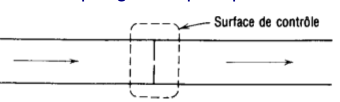
\includegraphics[scale=0.55]{ch5/image7.png}
	\captionof{figure}{ }
\end{center}
La détente augmente l'énergie cinétique mais souvent faible de sorte que 
$h_e\approx h_s$. La variation de température à travers la vanne est 
caractérisée par le coefficient de Joule-Thomson 
\begin{equation}
\mu_J = \left(\frac{\partial T}{\partial p}\right)_h
\end{equation}
S'il est positif, la température diminue à travers la vanne et inversement.



\section{Systèmes uniformes avec écoulement uniforme}
On va ici considérer un autre modèle simplifié qui possède les hypothèses 
suivantes :
\begin{enumerate}
\item Frontière immobile.
\item Propriété peuvent varier dans le temps, mais uniformément dans le 
système.
\item Propriété des sections $e$ et $s$ constantes dans le temps, mais les 
débits peuvent varier.
\end{enumerate}
Les équations sont modifiée comme tel :
\begin{equation}
\frac{dm_O}{dt} + \sum \dot{m_s}-\sum \dot{m_e}=0
\end{equation}
\begin{equation}
\frac{d}{dt}\left[\underbrace{m\left(u+\frac{c^2}{2}+gz\right)}_{U+E_{cin}+
E_{pot}}\right]_O + \sum\dot{m_s}\left(h+\frac{c^2}{2}+gz\right)_s-
\sum\dot{m_e}\left(h+\frac{c^2}{2}+gz\right)_e = \dot{Q}+\dot{W}
\end{equation}
Après intégration entre un état initial 1 et un état final 2 : 
\begin{equation}
m_2-m_1 + \sum m_s - \sum m_e = 0
\end{equation}
\begin{equation}
m_2\left(u_2+\frac{c_2^2}{2}+gz_2\right)-m_1\left(u_1+\frac{c_1^2}{2}+gz_1
\right)+\sum m_s\left(h_s\frac{c_s^2}{2}+gz_s\right)-\sum m_e\left(h_e\frac{
c_e^2}{2}+gz_e\right) = Q_0+W_0
\end{equation}
où $m_s$ et $m_e$ sont respectivement la masse totale ayant traversé les sections
d’entrée et de sortie, et $Q_O$ et $W_O$ les chaleur et travail reçus par le système au
cours de la transformation.












